\section{System Design Overview}

A search engine is a system that allows users to search for information on the internet. It consists of two main components: a crawler and a search engine. The crawler is responsible for collecting data from the internet, while the search engine is responsible for searching and displaying that data.

Since we are a team of two, we decided to split the work into two parts: one person will work on the crawler and the other person will work on the search engine. This way, we can work in parallel and complete the project faster.

\subsection{Crawler}

We both started by crawling our own universities, mine being INSA Lyon in France. I used \textbf{Selenium} to send requests and \textbf{BeautifulSoup} to parse the HTML content. \textbf{Selenium} was used because INSA Lyon's website is a single page application that only allows users to search people by name, as shown in \autoref{fig:insa_results_page}. This means that we cannot scrape the entire list of people from the website, but we can search for them by name. In the end, to get the full list of professors, I had to search through (with a rate limit to maintain politness) every two lettter combination of the alphabet (from "aa", "ab", "ac", ..., "zz") and store the results in a CSV file. Then clean it up by removing duplicates, students and staff.

\begin{figure}[ht]
	\centering
	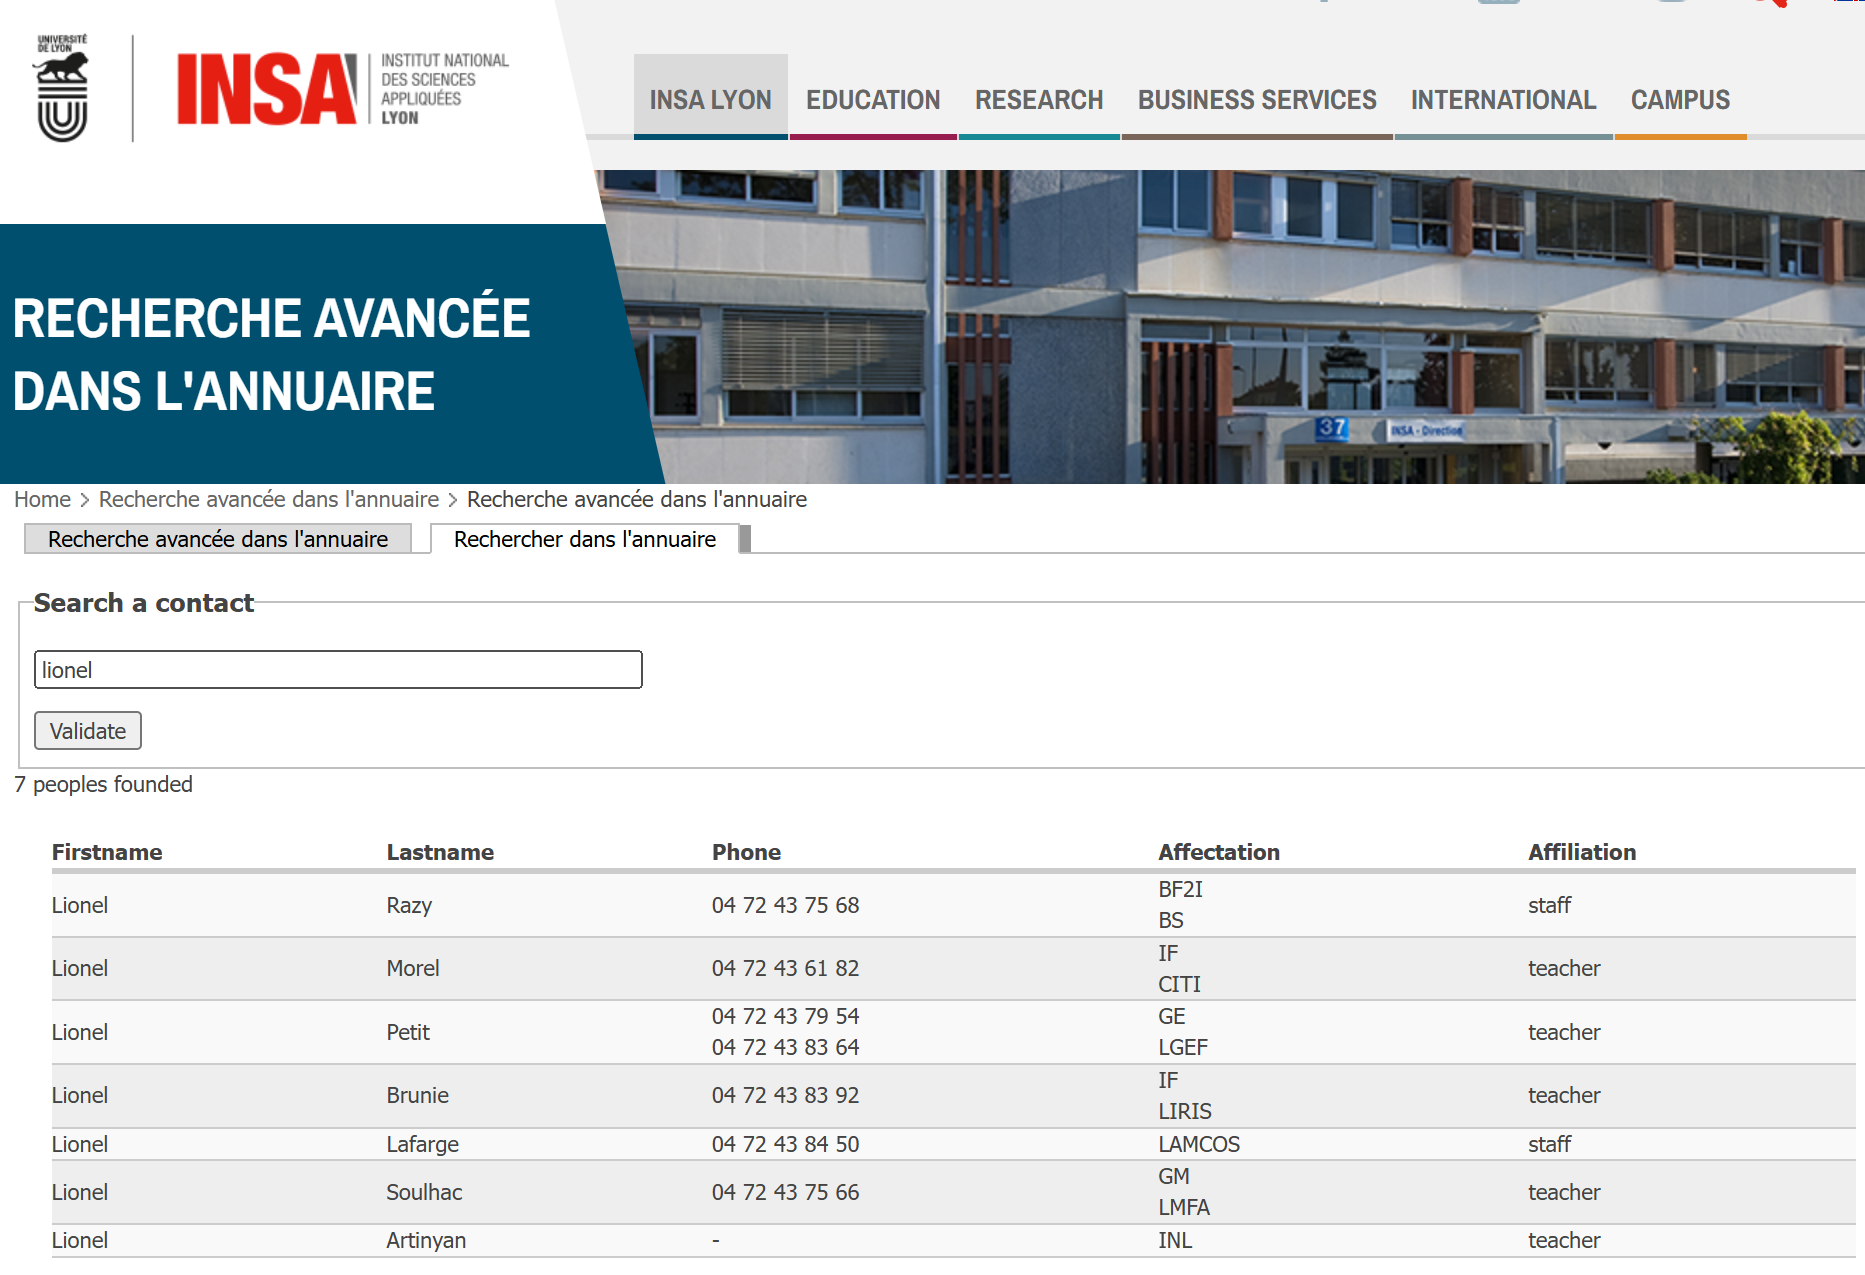
\includegraphics[width=0.7\textwidth]{insa-results-page.png}
	\caption{INSA Lyon's Results Page}
	\label{fig:insa_results_page}
\end{figure}

Now that I had data from my university, I wanted to start designing the layout of the search engine. I wanted to have a simple and clean design that would allow users to easily search for professors

\subsection{Search Engine}

I started by looking at different people search engines: LinkedIn, Instagram, Facebook, etc. I wanted to see how they display the results and what information they show. I also looked at different search engines such as Google to see how they display the results. Since the type of data we are dealing with is mostly related to the professors themselves, I wanted to display the name, title, and university of the professor as well as the picture if available. Therefore, I greatly inspired my design on LinkedIn's search results page (\autoref{fig:linkedin_results_page}~\cite{linkedin2025} and \autoref{fig:sorgle_results_page}) and its profile page (\autoref{fig:linkedin_profile_page}~\cite{linkedin2025} and \autoref{fig:sorgle_profile_page}).

\begin{figure}[ht]
	\centering
	\begin{minipage}{0.48\textwidth}
		\centering
		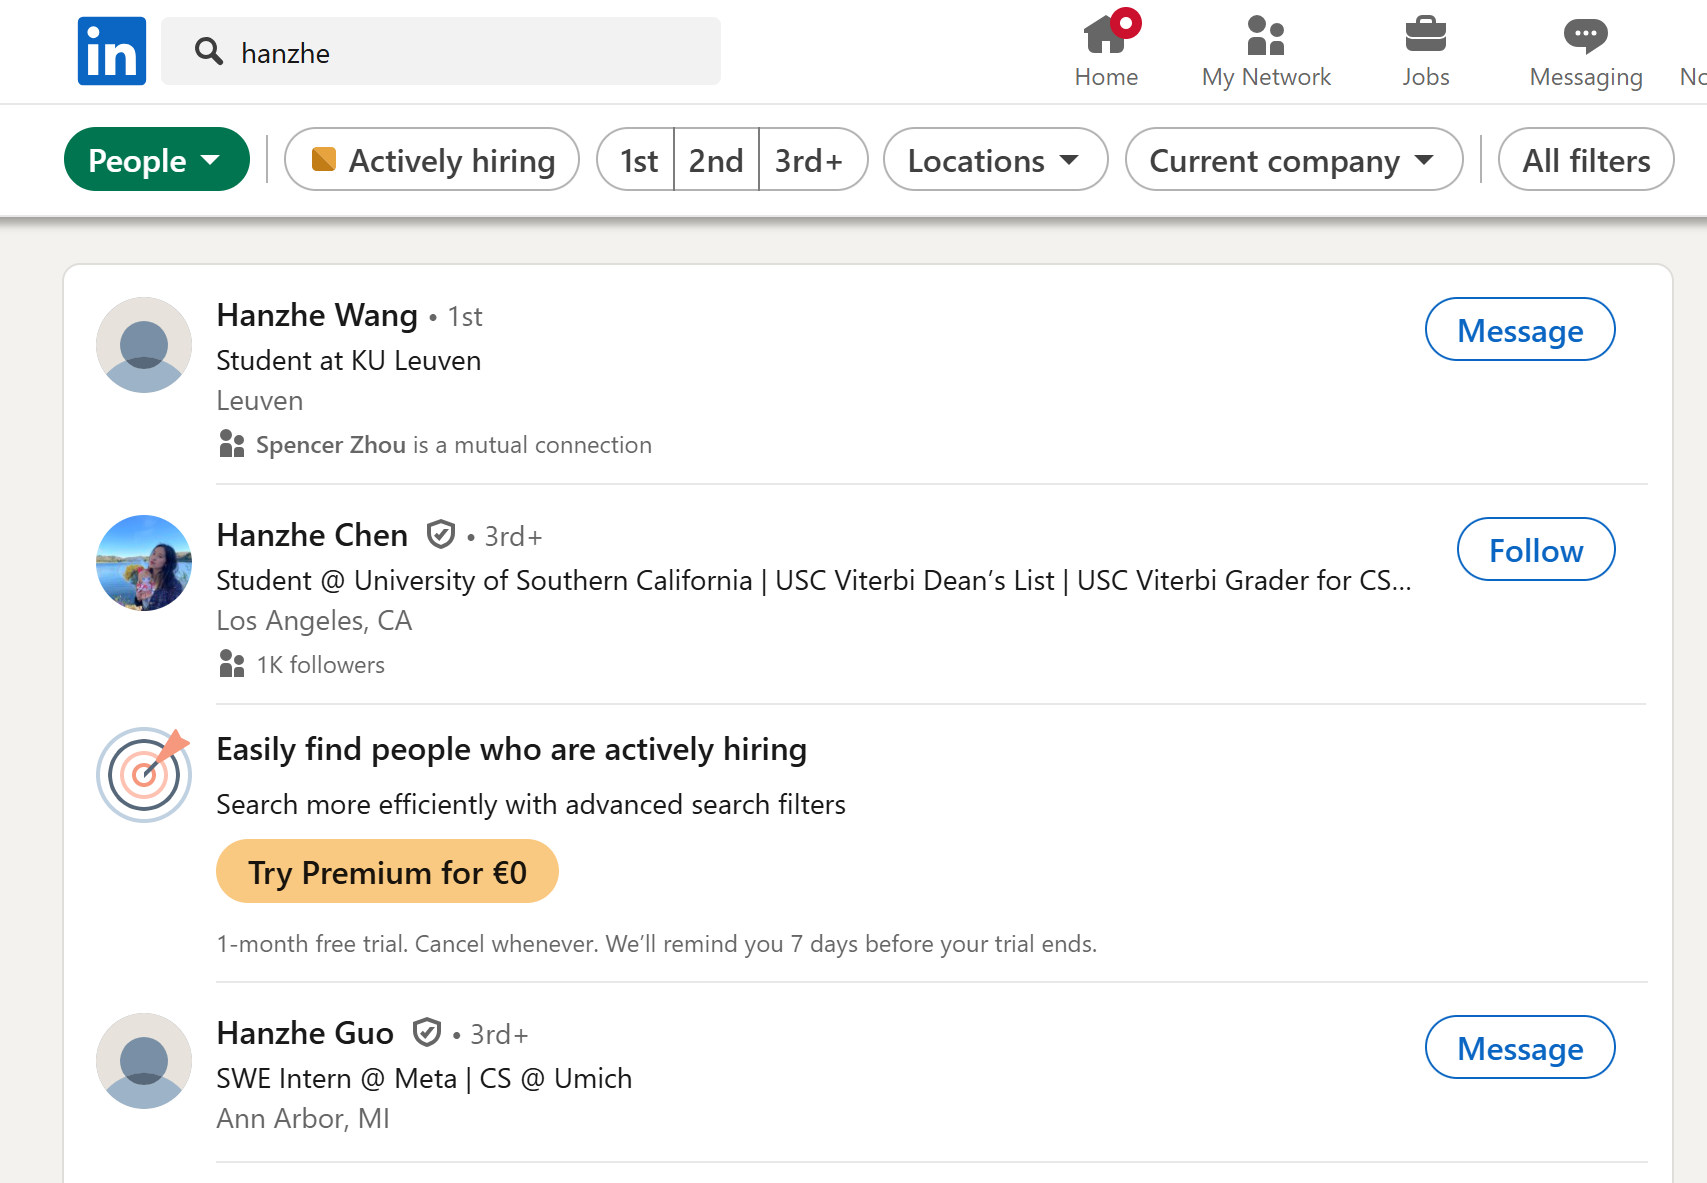
\includegraphics[width=\textwidth]{linkedin-results-page.png}
		\caption{LinkedIn Results Page \cite{linkedin2025}}
		\label{fig:linkedin_results_page}
	\end{minipage}\hfill
	\begin{minipage}{0.48\textwidth}
		\centering
		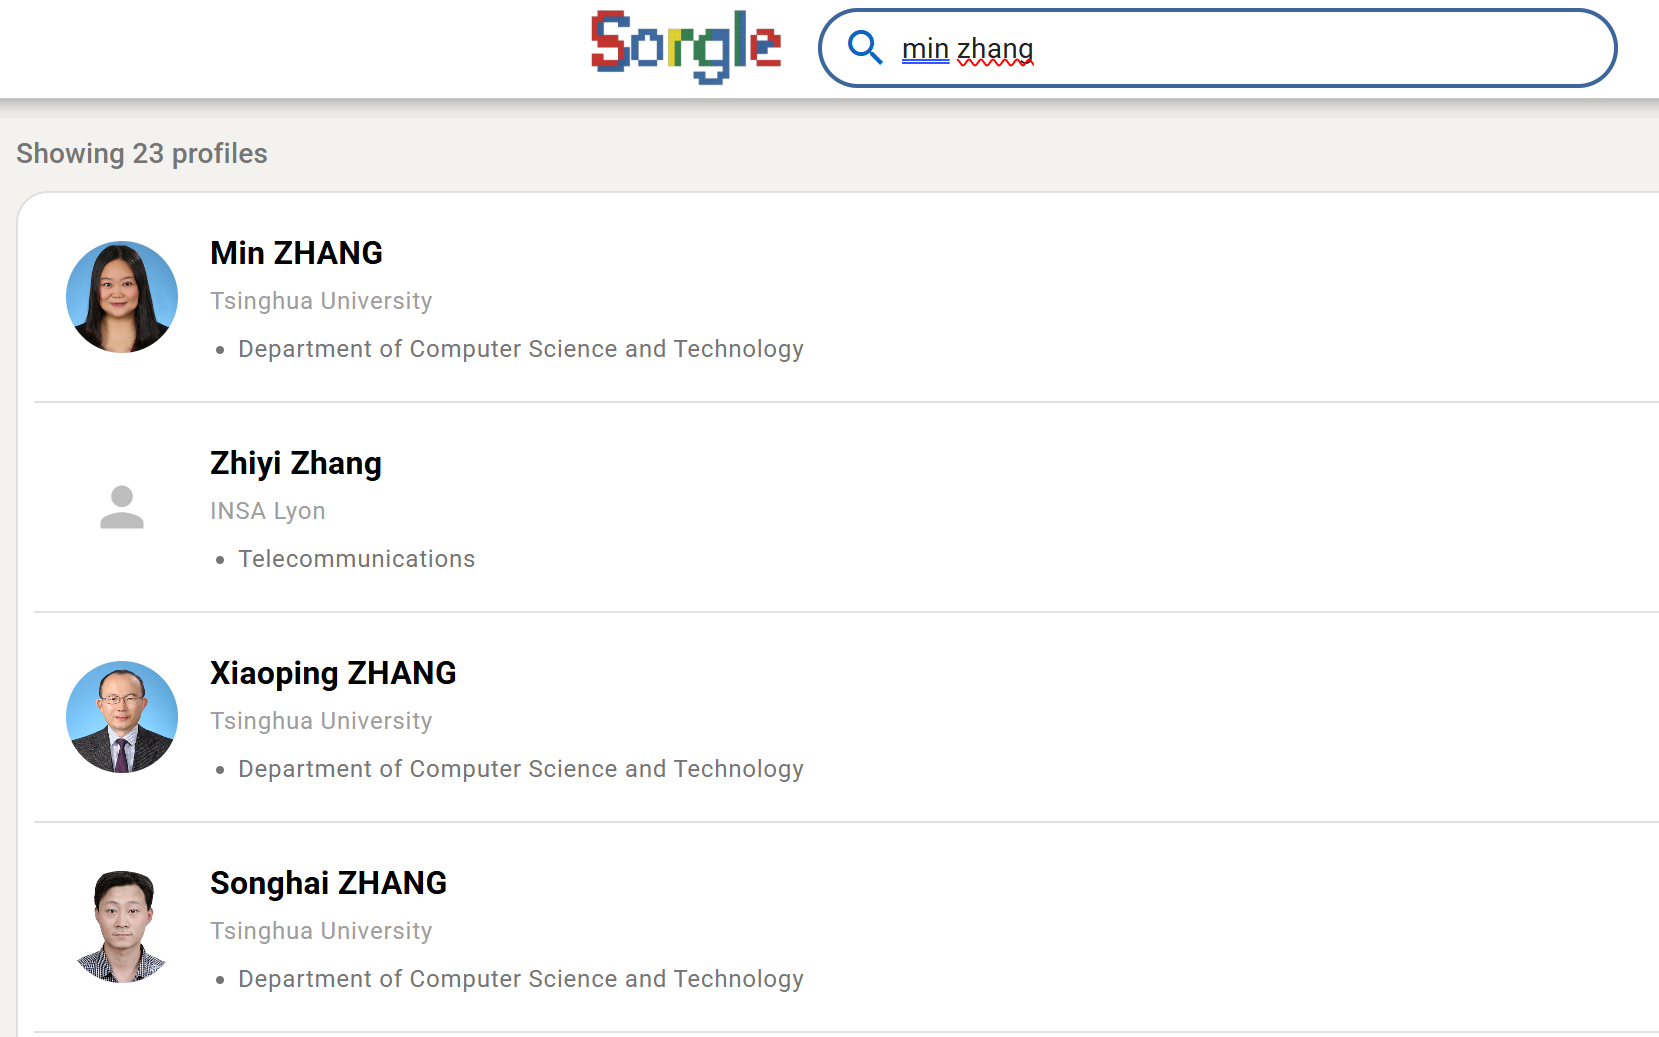
\includegraphics[width=\textwidth]{sorgle-results-page.png}
		\caption{Sorgle Results Page}
		\label{fig:sorgle_results_page}
	\end{minipage}
\end{figure}

\begin{figure}[ht]
	\centering
	\begin{minipage}{0.48\textwidth}
		\centering
		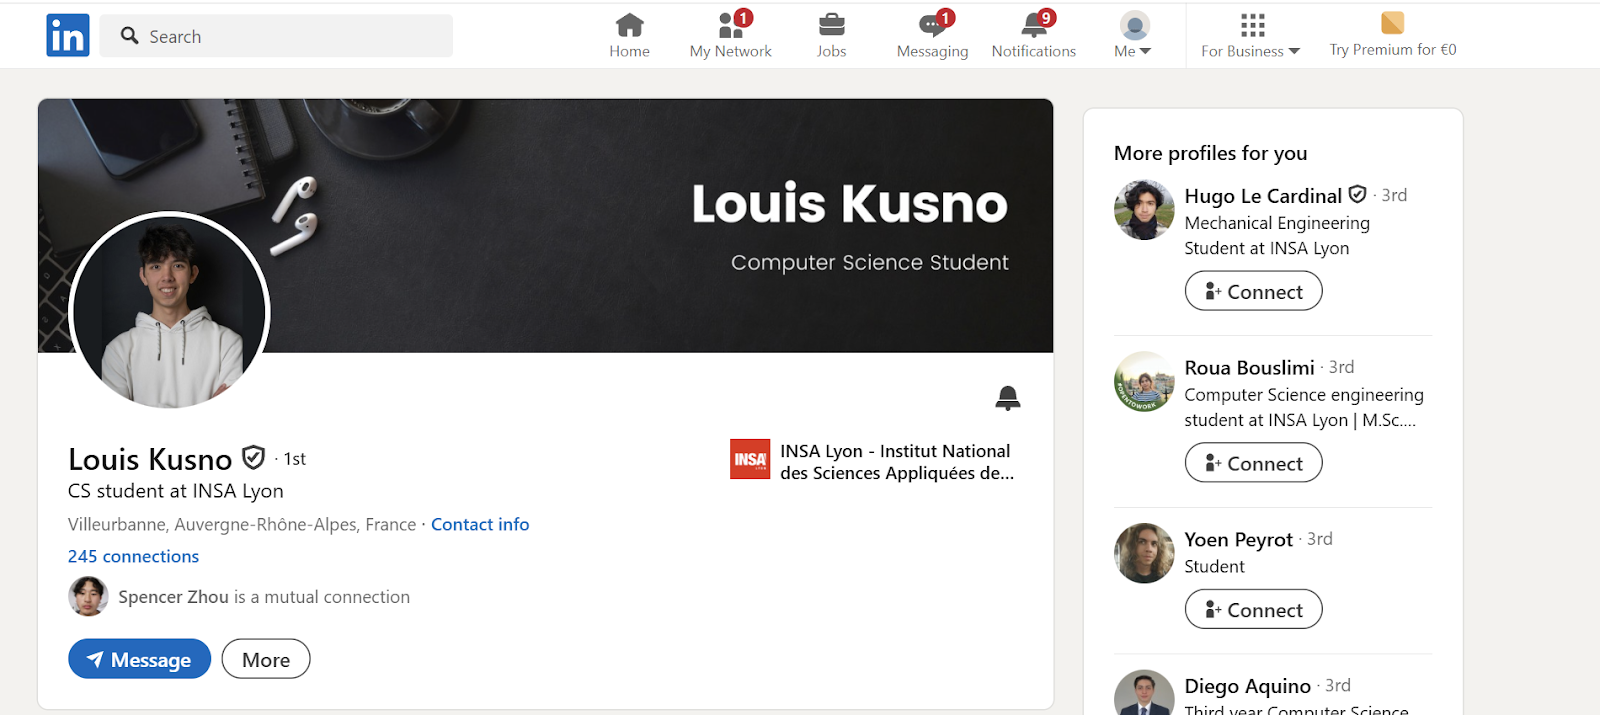
\includegraphics[width=\textwidth]{linkedin-profile-page.png}
		\caption{LinkedIn Profile Page \cite{linkedin2025}}
		\label{fig:linkedin_profile_page}
	\end{minipage}\hfill
	\begin{minipage}{0.48\textwidth}
		\centering
		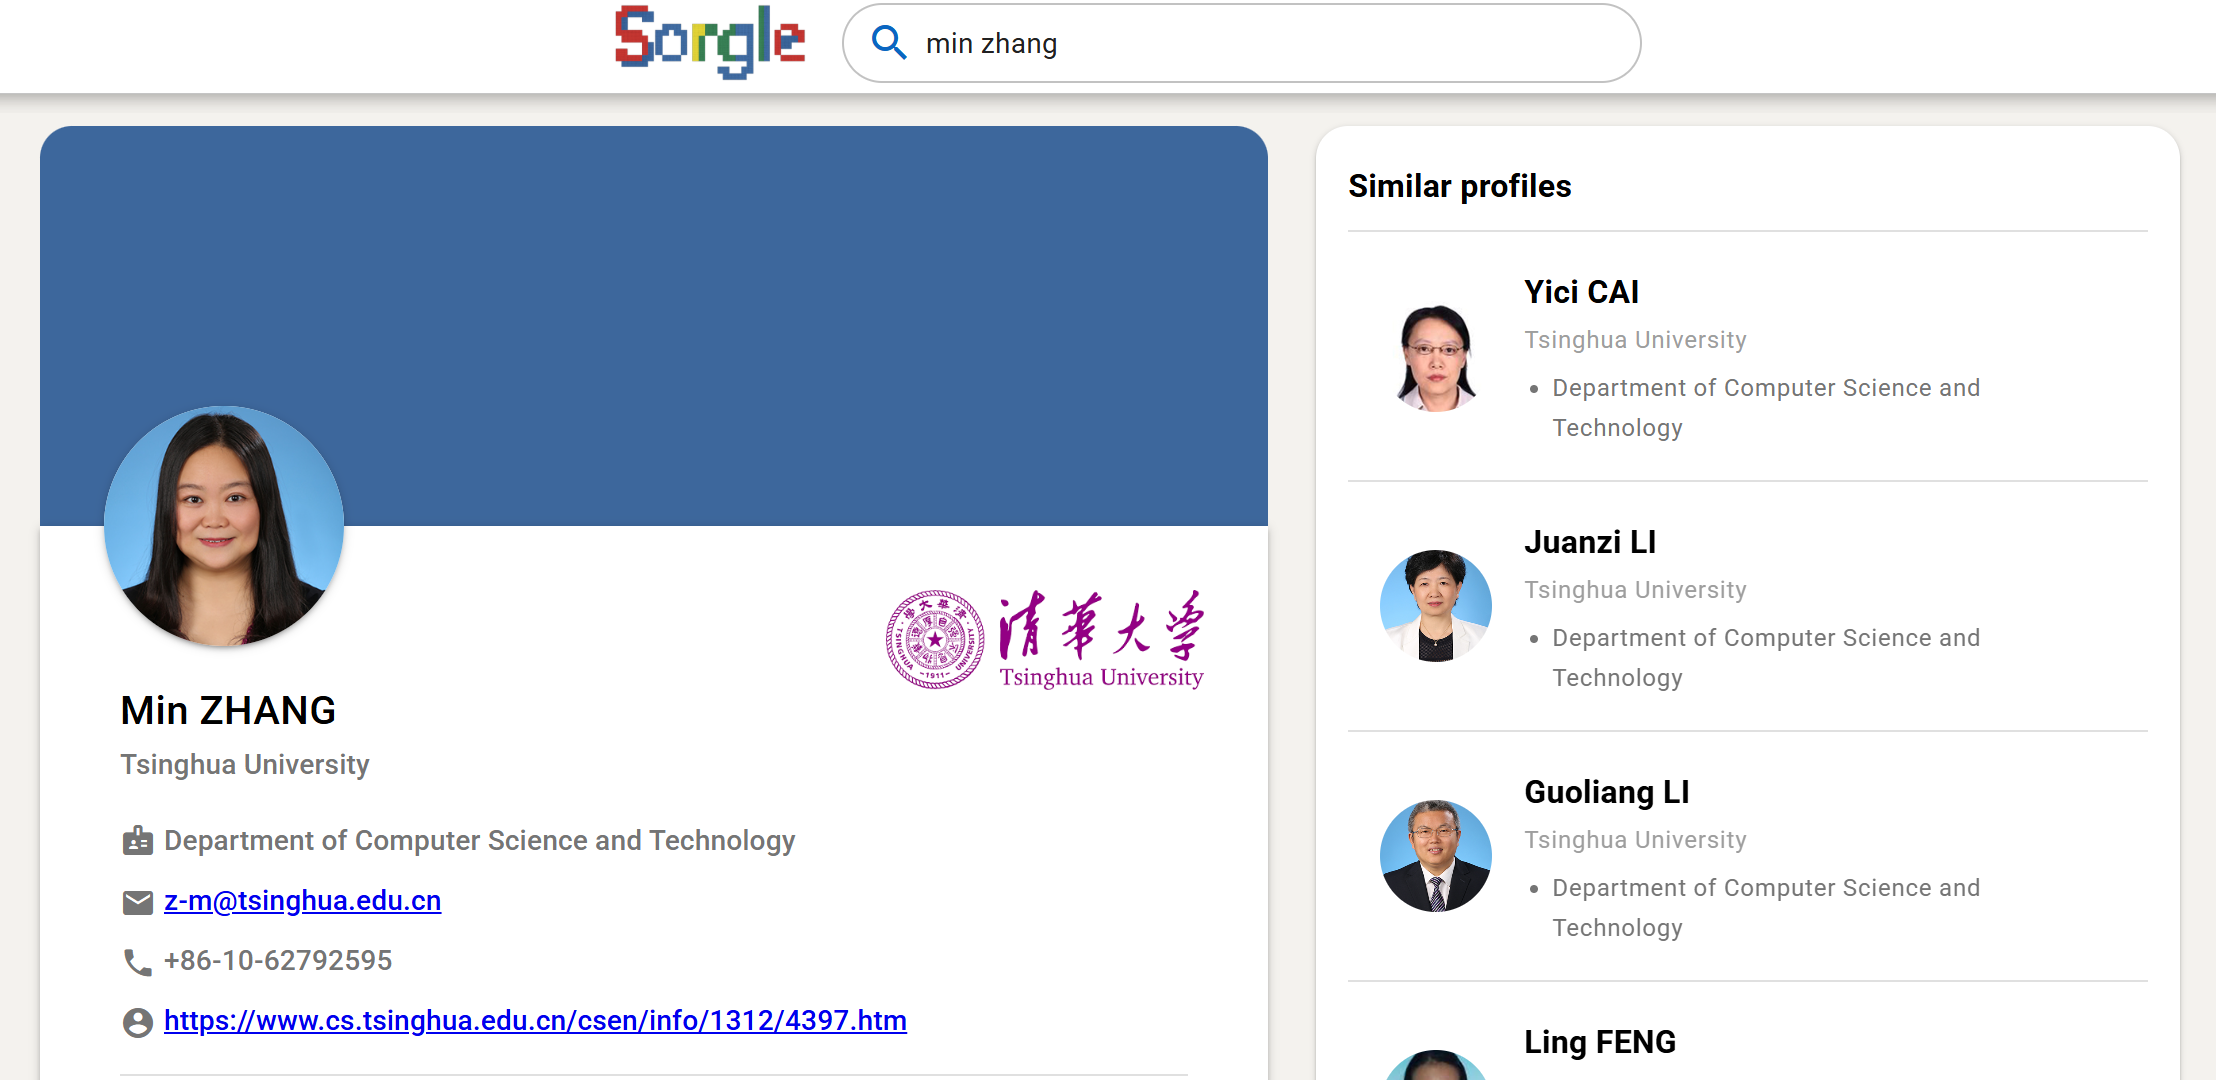
\includegraphics[width=\textwidth]{sorgle-profile-page.png}
		\caption{Sorgle Profile Page}
		\label{fig:sorgle_profile_page}
	\end{minipage}
\end{figure}

For the results page, I wanted to keep the design simple and clean, with a search bar at the top and the results displayed below it. I kept the information display very brief; the name, university and department because this is the data that all profiles have in common. I also really liked LinkedIn's color scheme. Even thought I set all my apps to dark mode, I think that light mode allows for a better looking website.

For the profile page, I wanted to display more information about the professor, basically all the information that I could scrape from the university's website. This includes:
\begin{itemize}
	\item Name
	\item University
	\item Department
	\item Profile picture
	\item Phone number
	\item Functions
	\item ORCID
	\item Bio
\end{itemize}

To display this information wihtout clutering the screen too much, I used logos that could best describe each field. Next, I really liked the idea of having similar profiles. This fills in the empty space on the right side of the page and allows users to use the search engine more efficiently (essentially increasing retention rate).

Lastly, the main page was inspired by Google's main page, this is coherent with my goal of having a simple and clean design.

\begin{figure}[ht]
	\centering
	\begin{minipage}{0.48\textwidth}
		\centering
		
\includegraphics[width=\textwidth]{google-main-page.png}
		\caption{Google Main Page \cite{google2025}}
		\label{fig:google_main_page}
	\end{minipage}\hfill
	\begin{minipage}{0.48\textwidth}
		\centering
		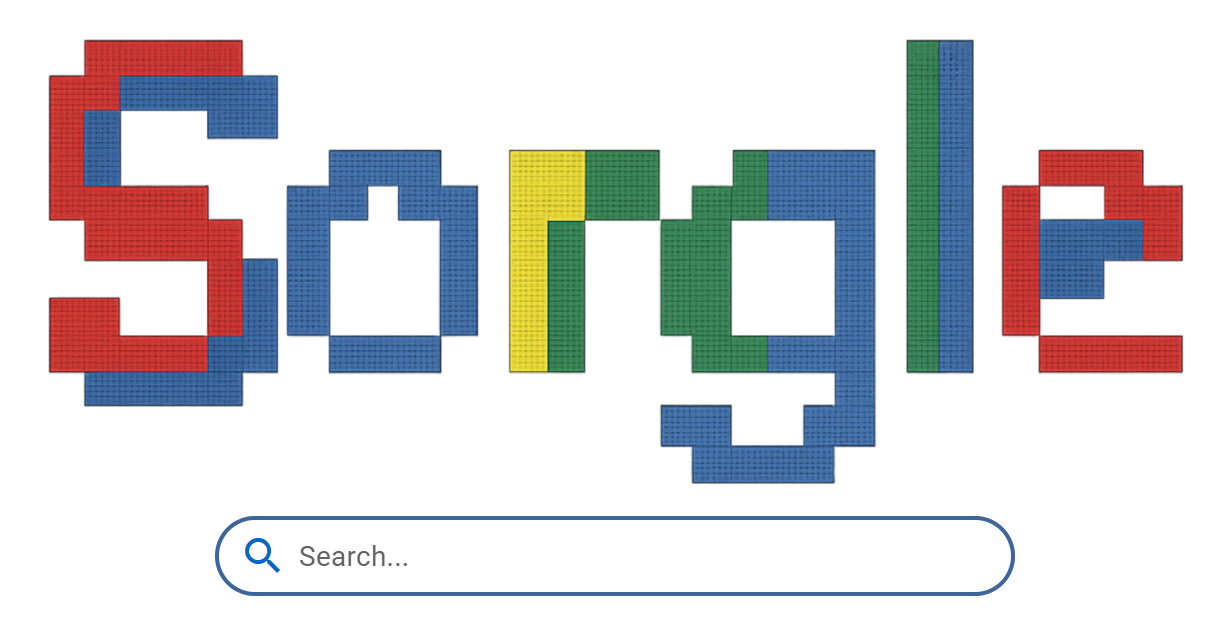
\includegraphics[width=\textwidth]{sorgle-main-page.png}
		\caption{Sorgle Main Page}
		\label{fig:sorgle_main_page}
	\end{minipage}
\end{figure}